\documentclass[11pt]{article}

\usepackage{graphicx}
\usepackage{subcaption}
\graphicspath{ {/home/macphej/jm.software/development/allosteric_signal/replica_ana/text/figures/} }

\begin{document}
\section*{Analysis of allosteric signals from MD simulations}
It has long been known that molecular dynamics is subject to statistical erorrs introduced by temporal and physical approximations associated with the simulation. While empirical force-fields represent the best approximation of molecular interactions within a protein, a pressing issue which faces the simulation community are questions of (1) reproducibility and (2) convergence.
\\
\\
In order to estimate the sampling precision, it is commonplace to perform a number of independent replicates. Having a quantifiable measure of the similarity in conformational space sampled by multiple replicates of the sample system is crucial for understanding the reproducibility of measurables extracted from an MD simulation. Simply, one needs to answer the following: 'how likely is it that I will sample the same conformational space, if I repeat an MD simulation seeded from the same structure multiple times?'. 
\\
\\
Secondly, ensuring convergence in biomolecular simulations is necessary to guarantee the quality of data. 'True convergence' is elusive to current computational capabilities given that to fully converge a protein would need to explore all possible conformational states, reversibly. This is difficult even for small peptide systems. As such, one can only hope to satisfy self-consistency checks. Several previous studies have shown that, even for a 1 $ms$ simulation of BPTI, satisfiying self-consistency checks early in the simulation are misleading because they fail to anticipate conformational changes, which occur later on in the simulation.
\\
\\
In order to interpret allosteric signals emerging from a structural alphabet analysis of MD simulation of PKM2, it was necessary to first determine the level of noise associated with the mutual information score by averaging over a number of simulations. We also reasoned that it would not be sensical to average over multiple replicates of a simulation if they explored different unique conformational space or were uniquely exposed to conformational traps. This necessitated a quantitative comparison in order to determine which ergodic sectors were explored by the simulation replicates. Secondly, to determine the confidence associated with the allosteric signals extracted from the simulations, we needed a quantitative estimate of convergence, using similarity (or dissimilarity) of the mutual information matrix as an input. 

\subsection*{Block covariance overlap method to measure egodicity of molecular dynamics simulation} 
The structural alphabet consists of 25 representative fragments of 4 consecutive C$\alpha$ atoms, such that the protein conformation is reduced to a string of $n-3$ letters. A column of this alignment describes all of the conformational states sampled by a protein fragment along the simulation trajectory. Corrleation of conformational changes in a pair of protein fragments $(i, j)$ was calculated as normalised mutual information:
\begin{equation}
I_{LL}^{n} (C_{i}:C_{j}) = \frac{I(C_{i}:C_{j}) - \epsilon (C_{i}:C_{j})}{H(C_{i}:C_{j})}
\end{equation}
When the ensemble of protein conformations originates from an MD simulation, each of the eigenvectors resulting from the diagonalization of the mutual information matrix, describes a collective mode of motion that is not linearly correlated with any other in the system. The extent of this motion is given by the corresponding eigenvalue. This an eigenvalue decomposition of the mutual information matrix is a good way of assessing to what degree two simulations sample the same 'allosteric information space'.
\\
\\
One way to quantify the overlap between two matrices, is to perform an eigenvalue decomposition and then to compute the direction cosine between the eigenvector matrices:
\begin{equation}
\Psi_{A:B} = \frac{1}{n} \sum_{i}^{n} \sum_{j}^{n} (\textbf{v}_{i}^{A} \cdot \textbf{v}_{i}^{B})^{2}
\end{equation}
Equation $2$ is fairly permissive as a convergence criterium because the magnitudes along eigenvectors of the different modes are not considered, only the direction of the vectors. To expand on this, we can weight the direction cosine measure by the magnitude along the respective eigenvectors:
\begin{equation}
\Omega_{A:B} = 1 - \lbrace \frac{\sum_{i=1}^{3N}(\lambda_{i}^{A} + \lambda_{i}^{B}) - 2 \sum_{i=1}^{3N} \sum_{j=1}^{3N} (\lambda_{i}^{A} \lambda_{i}^{B})^{0.5} (\textbf{v}_{i}^{A} \cdot \textbf{v}_{i}^{B})^{2}}{\sum_{i=1}^{3N}(\lambda_{i}^{A} + \lambda_{i}^{B})} \rbrace ^{0.5}
\end{equation}
where $\lambda^{A}$ and $\lambda^{B}$ denote the eigenvalues of the mutual information matrices for simulations A and B, and $N$ is the number of alpha carbon atoms in the calculations. We define this measure as the 'covariance overlap'.
\\
\\
The covariance overlap between two mutual information matrices
\subsection*{Test case 1: 10 ns MD simulation of deca-alanine in vacuum}
A 10 $ns$ simulation of a deca-alanine peptide in vacuum was used as a test system for examining the behaviour of the time-evolution of mutual information matrices derived from a structural-alphabet representation of the trajectory. In particular, we wanted to test the numerical behviour of the cosine content and covariance overlap with different eigenmodes used in the calculation. 
\begin{figure}[hbt]
\centering
\begin{subfigure}[b]{.24\linewidth}
    \centering
    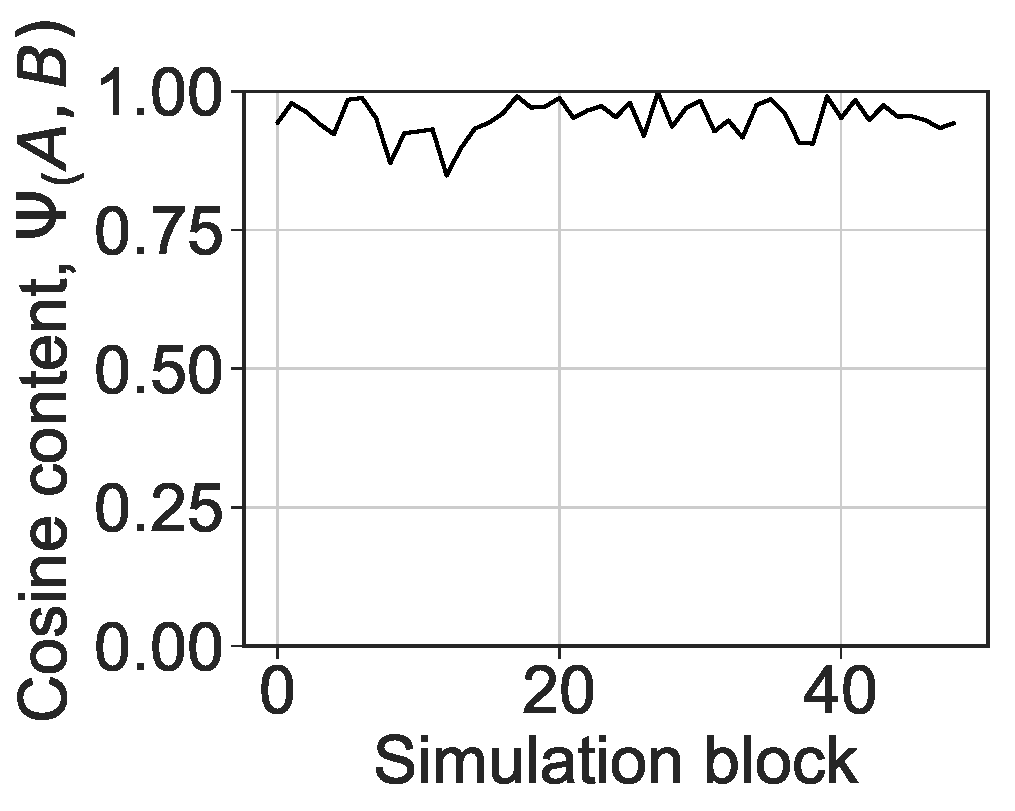
\includegraphics[width=.99\textwidth]{time_CosCont_n1.pdf}
    \caption{$E$ = 1}\label{fig:1a}
  \end{subfigure}%   
  \begin{subfigure}[b]{.24\linewidth}
    \centering
    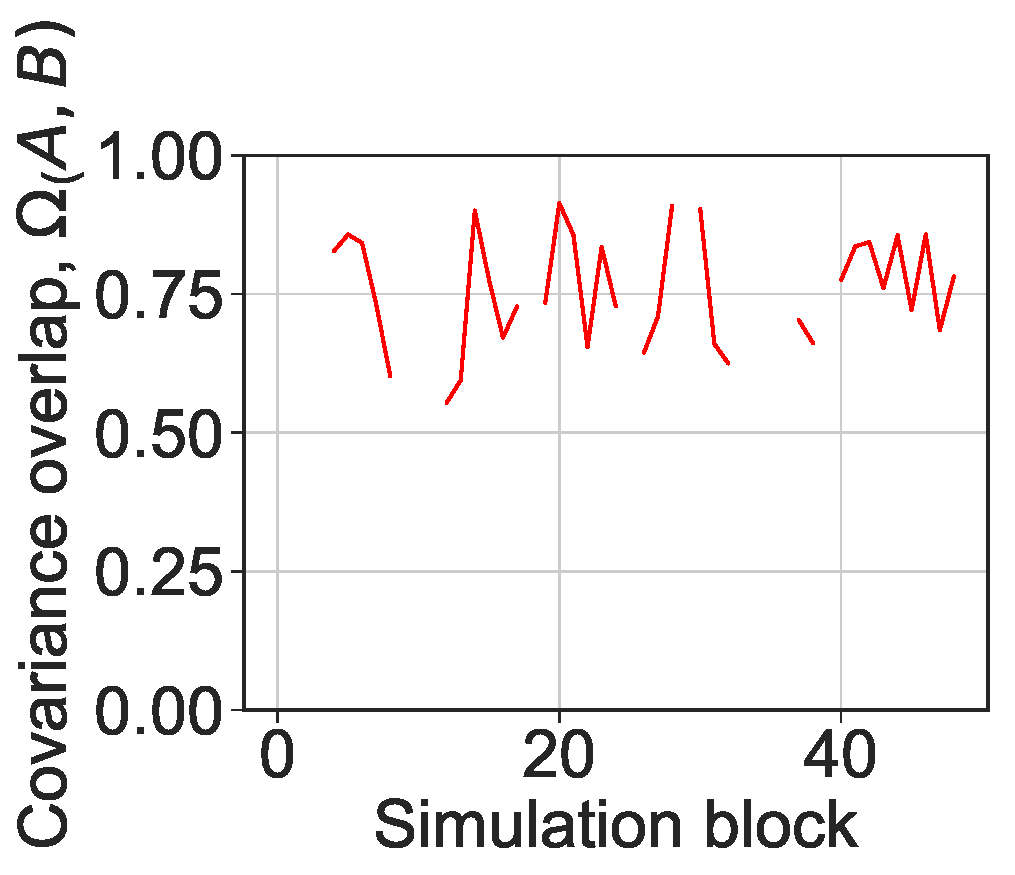
\includegraphics[width=.99\textwidth]{time_CovOver_n1.pdf}
    \caption{$E$ = 1}\label{fig:1b}
  \end{subfigure}%  
  \begin{subfigure}[b]{.24\linewidth}
    \centering
    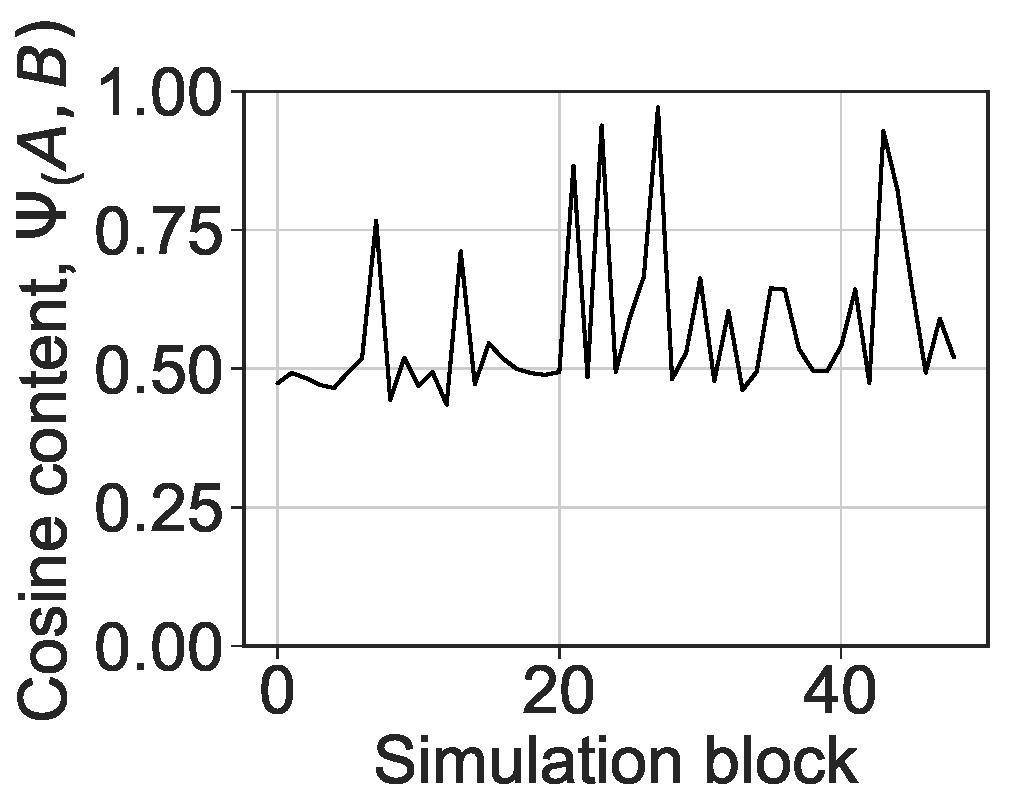
\includegraphics[width=.99\textwidth]{time_CosCont_n2.pdf}
    \caption{$E$ = 2}\label{fig:1c}
  \end{subfigure}%  
  \begin{subfigure}[b]{.24\linewidth}
    \centering
    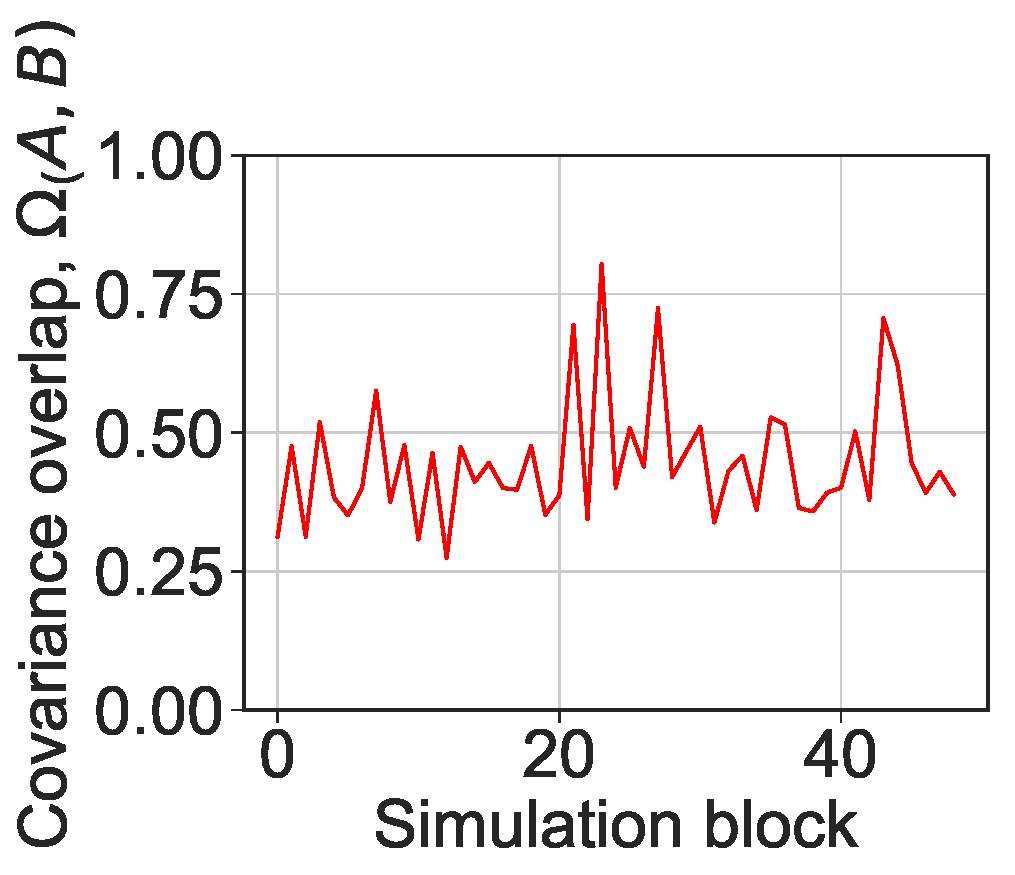
\includegraphics[width=.99\textwidth]{time_CovOver_n2.pdf}
    \caption{$E$ = 2}\label{fig:1d}
  \end{subfigure}\\%   
  \begin{subfigure}[b]{.24\linewidth}
    \centering
    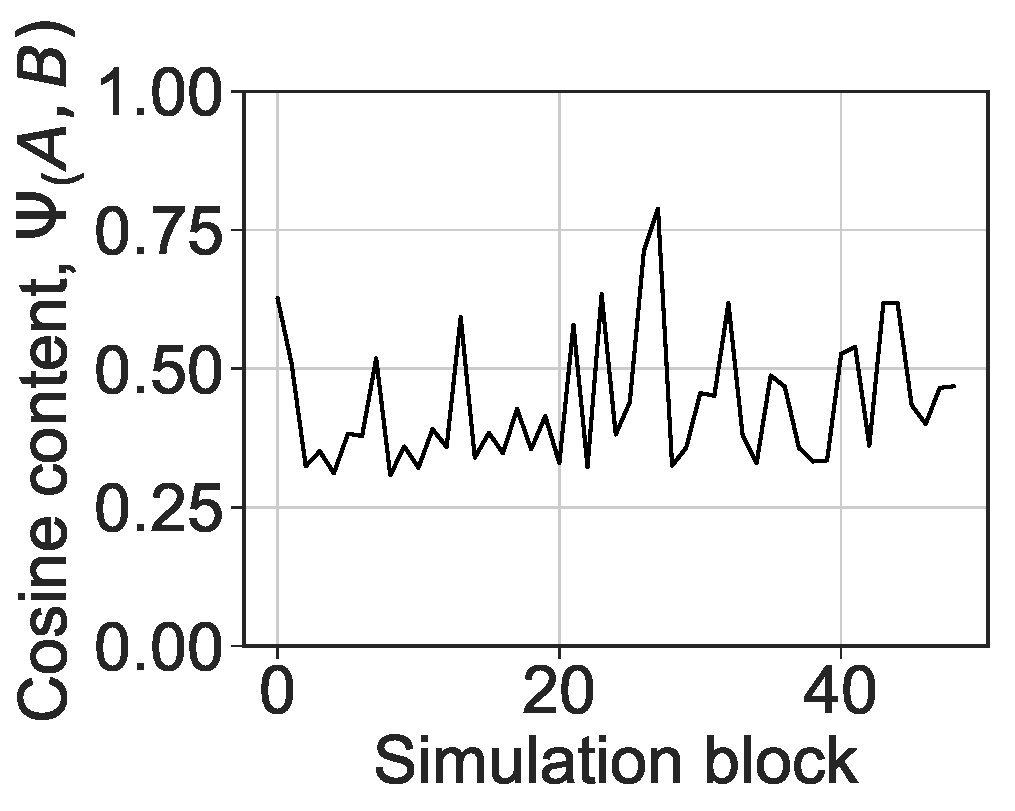
\includegraphics[width=.99\textwidth]{time_CosCont_n3.pdf}
    \caption{$E$ = 3}\label{fig:1e}
  \end{subfigure}%
  \begin{subfigure}[b]{.24\linewidth}
    \centering
    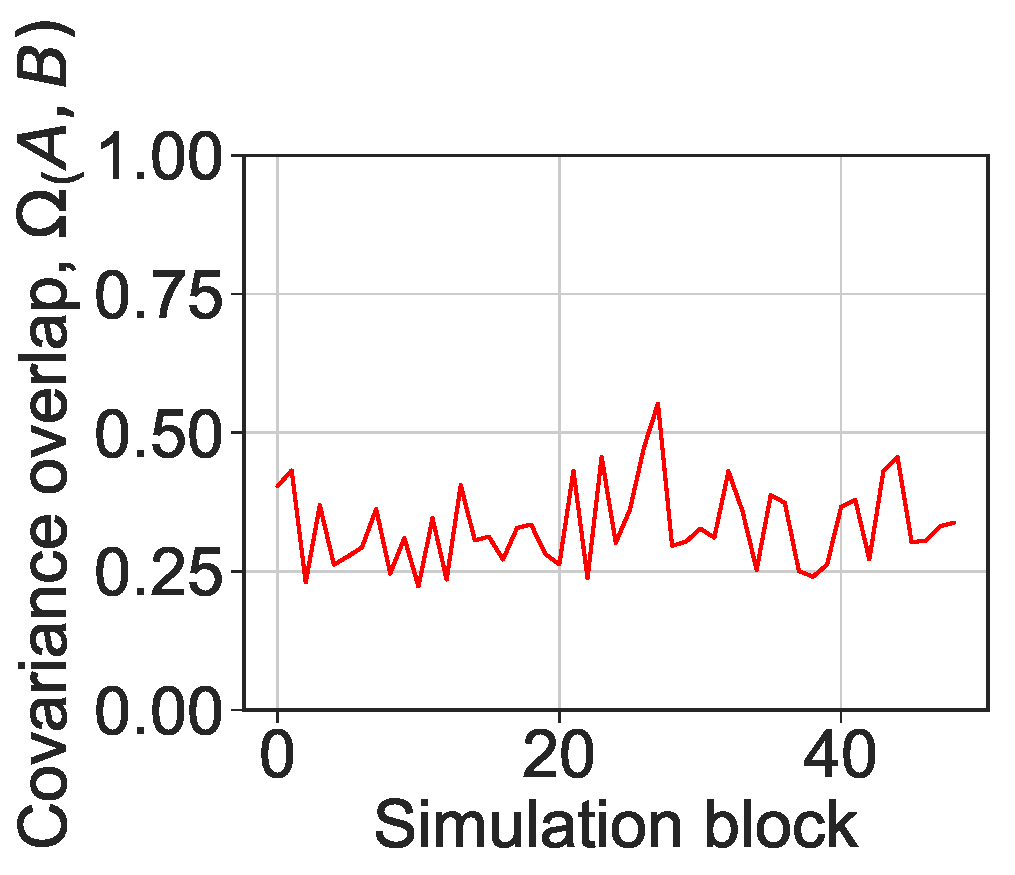
\includegraphics[width=.99\textwidth]{time_CovOver_n3.pdf}
    \caption{$E$ = 3}\label{fig:1f}
  \end{subfigure}%
  \begin{subfigure}[b]{.24\linewidth}
    \centering
    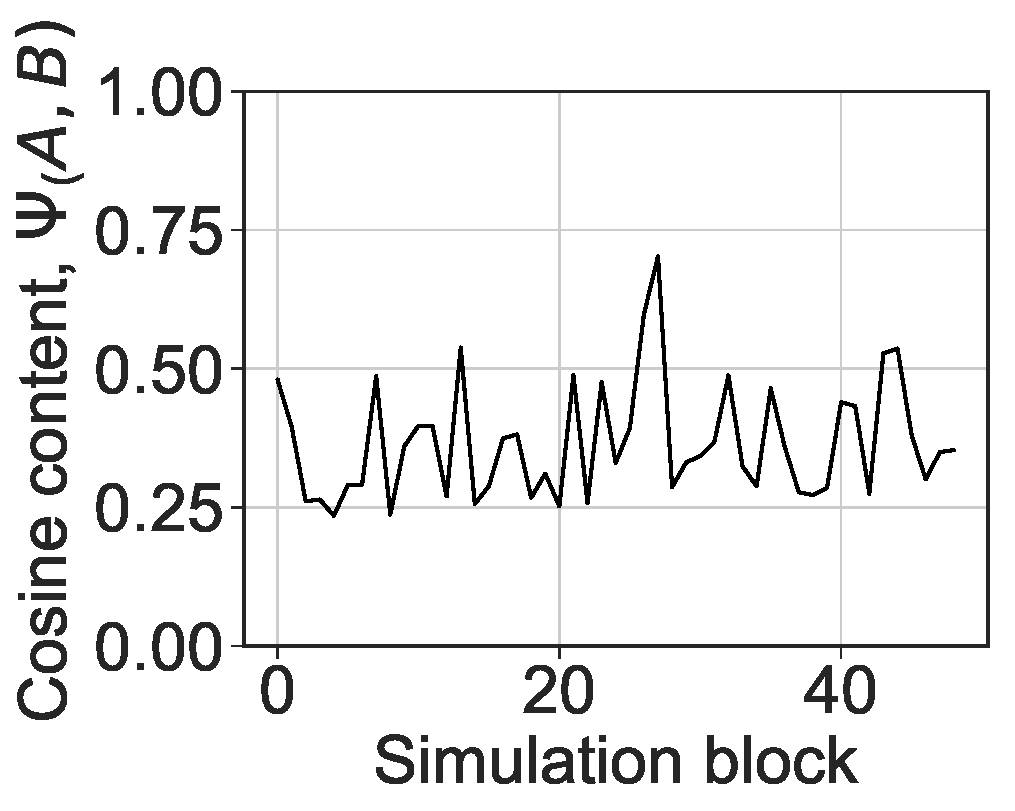
\includegraphics[width=.99\textwidth]{time_CosCont_n4.pdf}
    \caption{$E$ = 4}\label{fig:1g}
  \end{subfigure}%
  \begin{subfigure}[b]{.24\linewidth}
    \centering
    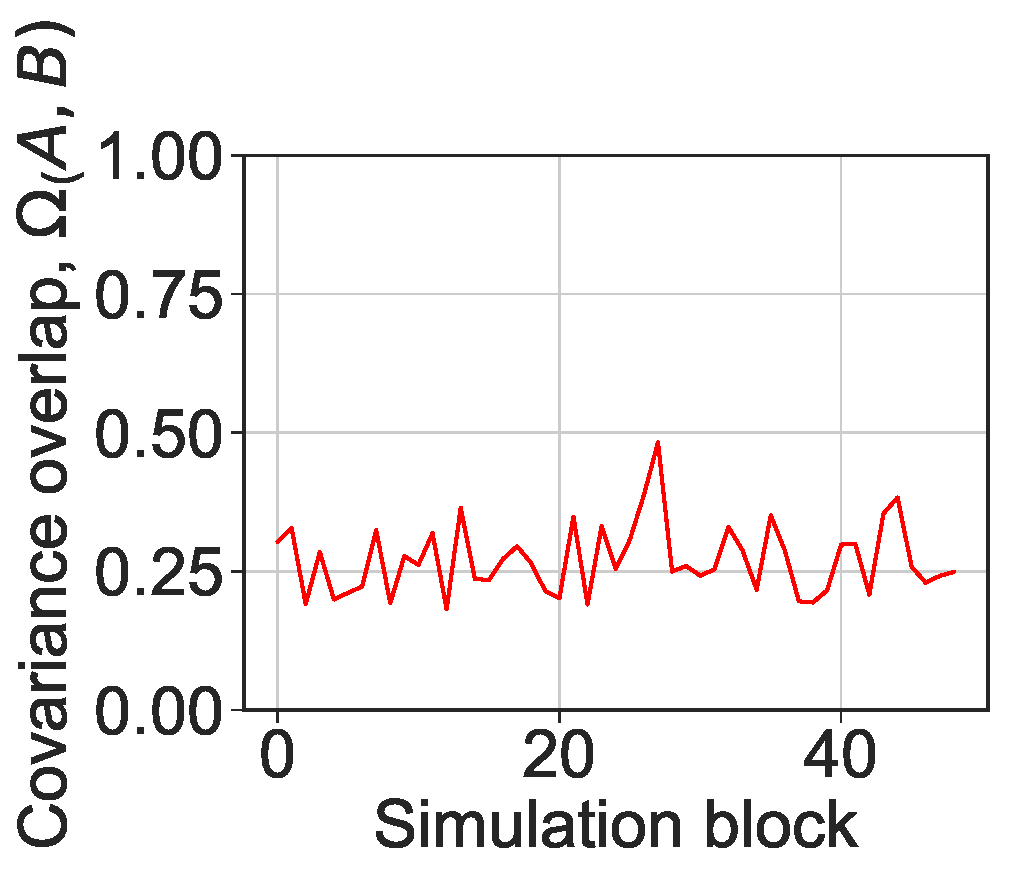
\includegraphics[width=.99\textwidth]{time_CovOver_n4.pdf}
    \caption{$E$ = 4}\label{fig:1h}
  \end{subfigure}\\%     
  \begin{subfigure}[b]{.24\linewidth}
    \centering
    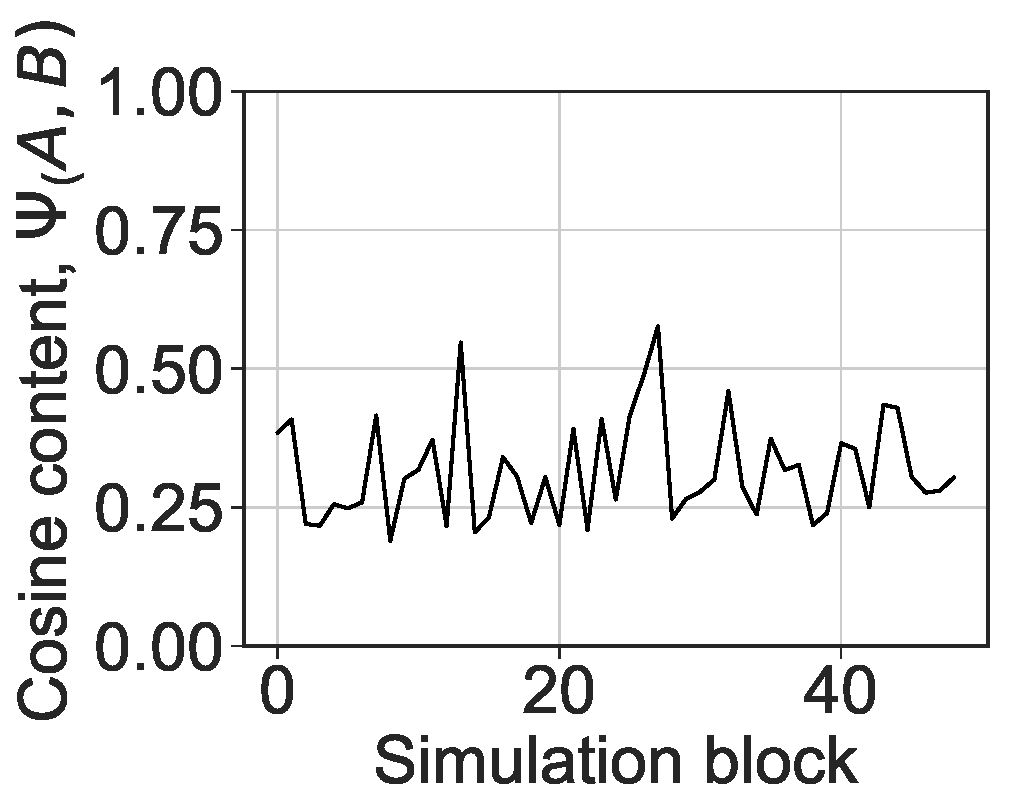
\includegraphics[width=.99\textwidth]{time_CosCont_n5.pdf}
    \caption{$E$ = 5}\label{fig:1i}
  \end{subfigure}%
  \begin{subfigure}[b]{.24\linewidth}
    \centering
    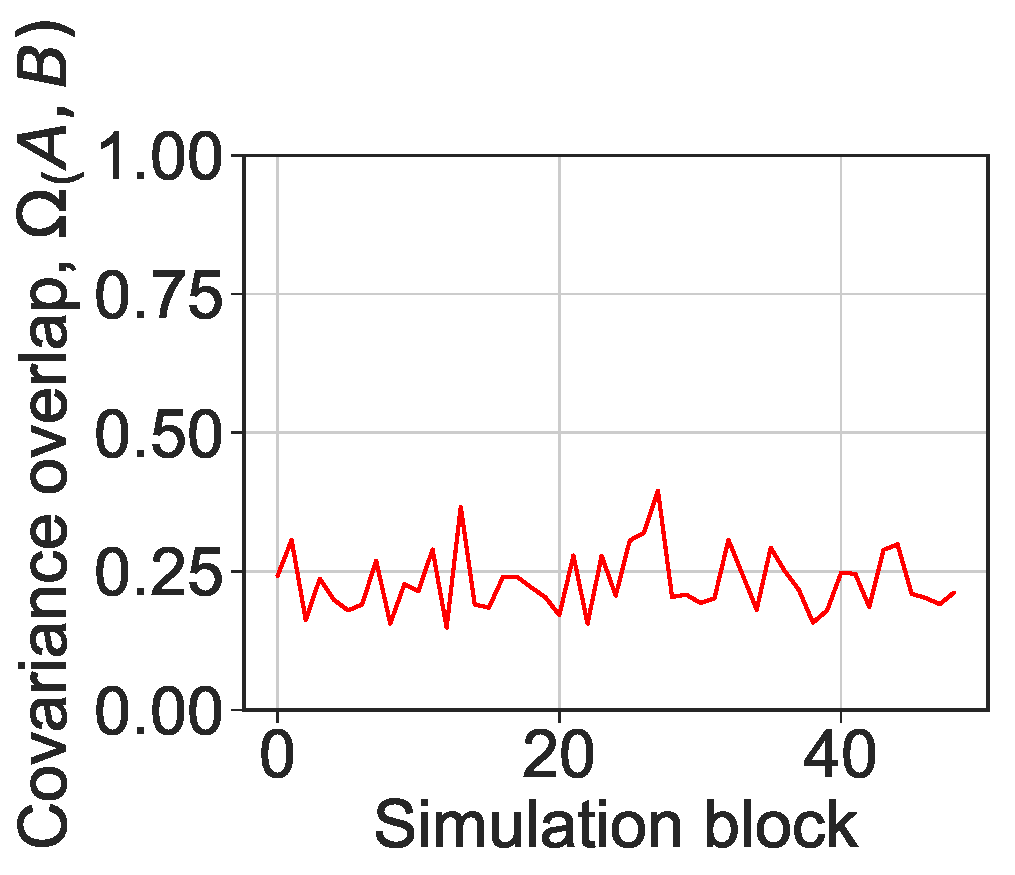
\includegraphics[width=.99\textwidth]{time_CovOver_n5.pdf}
    \caption{$E$ = 5}\label{fig:1j}
  \end{subfigure}%
  \begin{subfigure}[b]{.24\linewidth}
    \centering
    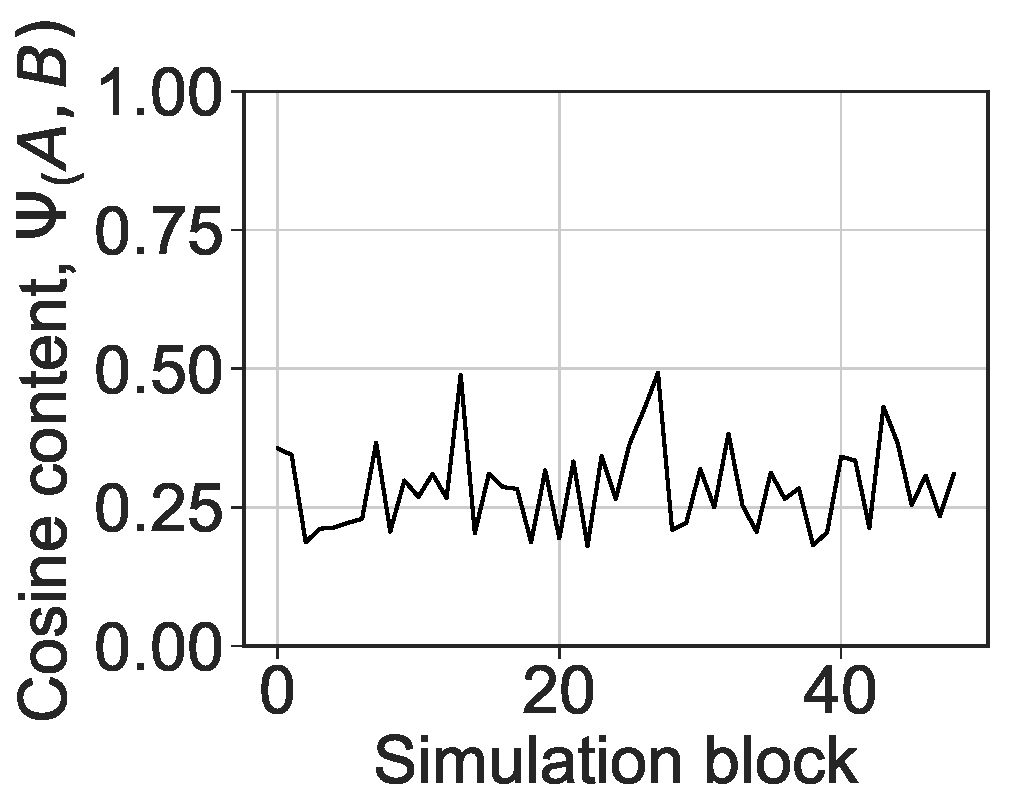
\includegraphics[width=.99\textwidth]{time_CosCont_n6.pdf}
    \caption{$E$ = 6}\label{fig:1k}
  \end{subfigure}%
  \begin{subfigure}[b]{.24\linewidth}
    \centering
    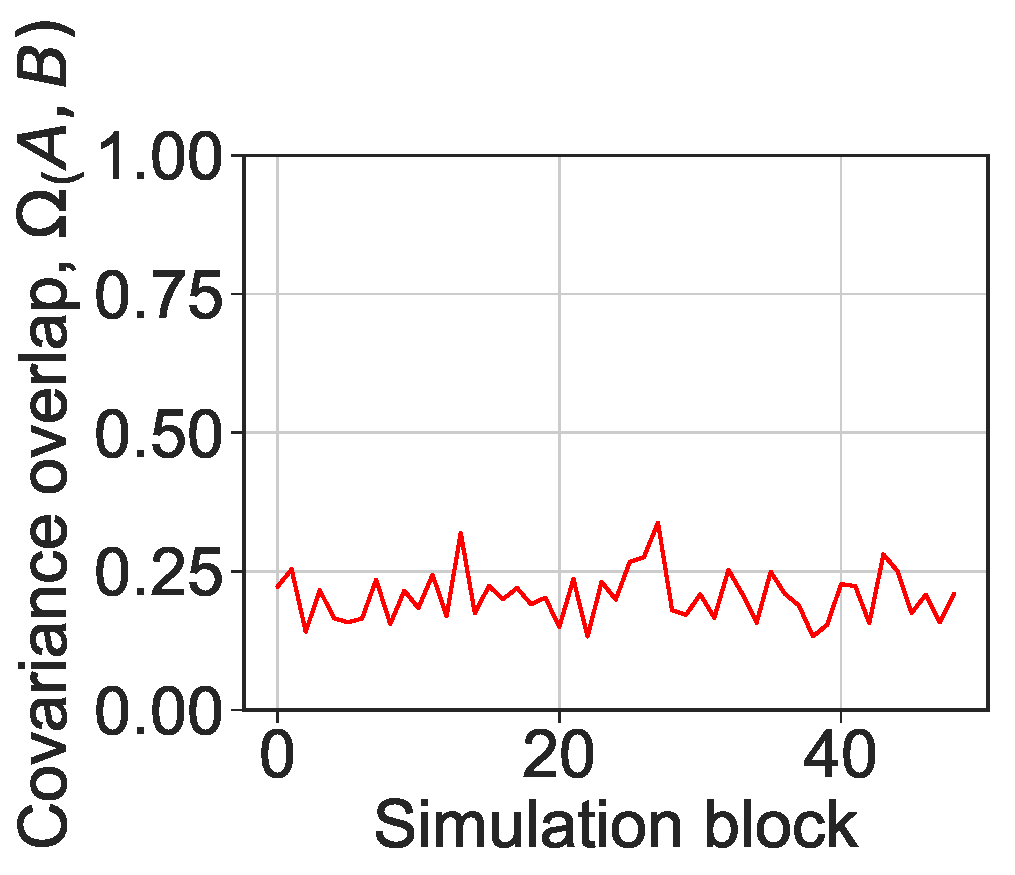
\includegraphics[width=.99\textwidth]{time_CovOver_n6.pdf}
    \caption{$E$ = 6}\label{fig:1l}
  \end{subfigure}\\%   
\caption{The numerical behaviour of spectral subspace overlap with different eigenmodes}\label{fig:1}
\end{figure}
The time evolution of both the cosine content and the covairance overlap decreases with increased numbers of eigenmodes included in the calculation. This is because a higher spectral variance is explicitly considered when more eigenmodes are summed over in equations (2) and (3). Also of note, the decreased subspace overlap converged after the first three eigenmodes. This convergent behaviour is consistent with the rapid decay in the eigenvalues, shown below.
\begin{figure}[!ht]
\centering
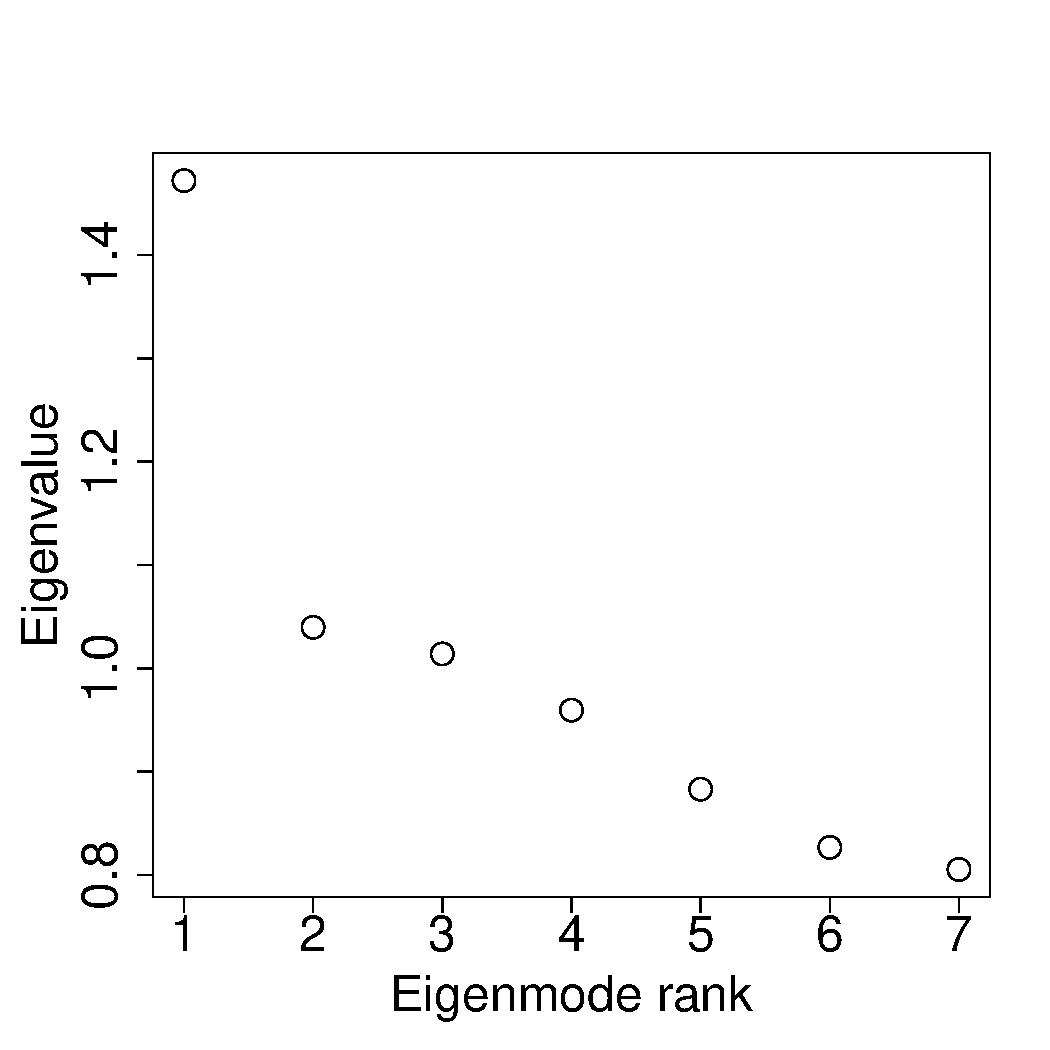
\includegraphics[scale=0.4]{eigenvariance.pdf}
\caption{Scree plot of eigenvalue distribution of mutual information matrix}\label{fig:2} 
\end{figure}
In this particular example of deca-alanine in vacuum for 10 $ns$ at 300 $K$ there is very little conformational motion in the peptide. This is reflected by the high degree of overlap between the trajectory blocks, shown in figure 1. Furthermore, figure 2 indicates that the first eigenmode represents a significant amount of the positional variance in the trajectory and that subsequent eigenmodes contain negligable variance. To this point, the convergence in the subspace overlap measures $\omega$ and $\Psi$ result from increased variance included in the measure. This raises an important statistical question: which eigenmodes are statistically signficant?
\\
\\
Going back to the initial problem of detecting subspace sampling of MD trajectories it became obvious that the deca peptide, which a good test case for assessing the numerical behaviour of $\omega$ and $\Psi$, was not very useful for interrogating whether or not the mutual information was sensitive to global conformational changes. To investigate this problem, we measured the subspace overlap of a more complex system - monomeric PKM2 bound to Tepp-46.
\subsection*{Test case 2: 1 $\mu s$ MD simulation of monomeric PKM2 bound to Tepp-46}
We have seen that monomeric PKM2 undergoes a significant ligand-dependent conformational rearrangement upon binding Tepp-46. Particularly, the B-domain cap closes over the catalytic pocket when the allosteric activator is bound and remains in an 'open' conformation when in the 'apo' state. When Tepp-46 is bound, the B-domain cap closes at around 150 $ns$ (not shown). Here, given that the protien undergoes a significant conformational rearrangement during the simulation we hypothesised that it would be a good test system to determine whether global conformational changes were accounted for my local correlations in the fragment scheme.
\\
\\
We started by measuring the subspace overlap for different numbers of eigenmodes, to investigate whether local correlations are sensitive to global conformational changes. 
\begin{figure}[hbt]
\centering
\begin{subfigure}[b]{.24\linewidth}
    \centering
    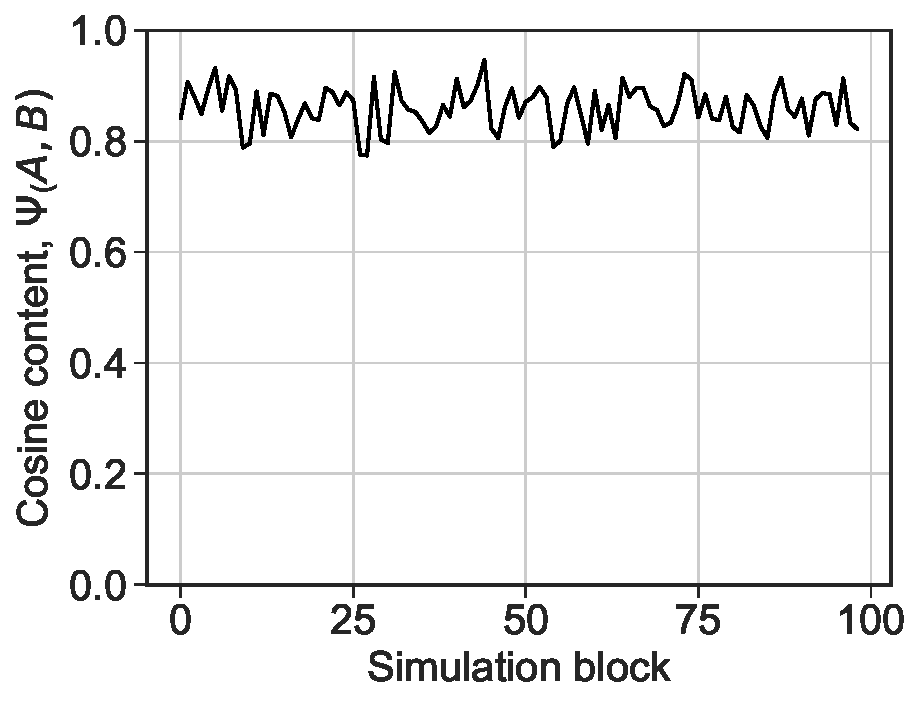
\includegraphics[width=.99\textwidth]{time_CosCont_E1.pdf}
    \caption{$E$ = 1}\label{fig:1a}
  \end{subfigure}%   
  \begin{subfigure}[b]{.24\linewidth}
    \centering
    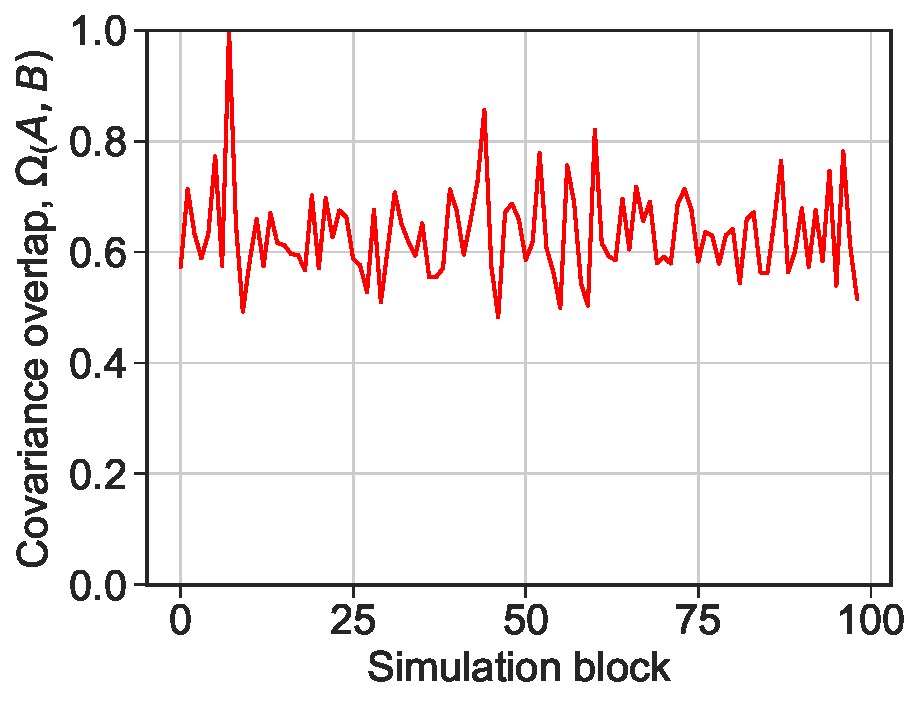
\includegraphics[width=.99\textwidth]{time_CovOver_E1.pdf}
    \caption{$E$ = 1}\label{fig:1b}
  \end{subfigure}%  
  \begin{subfigure}[b]{.24\linewidth}
    \centering
    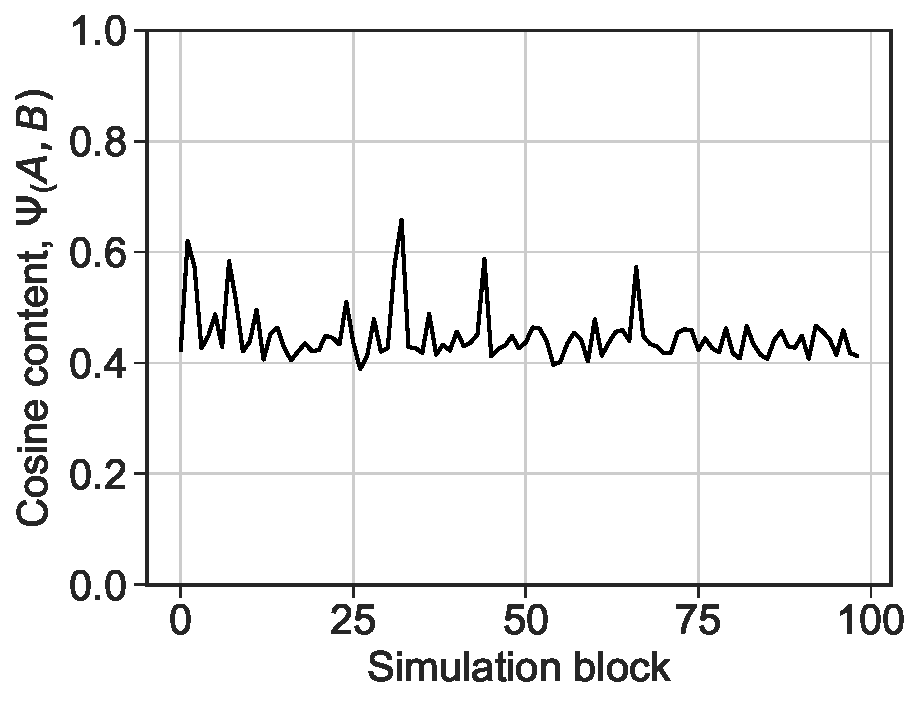
\includegraphics[width=.99\textwidth]{time_CosCont_E2.pdf}
    \caption{$E$ = 2}\label{fig:1c}
  \end{subfigure}%  
  \begin{subfigure}[b]{.24\linewidth}
    \centering
    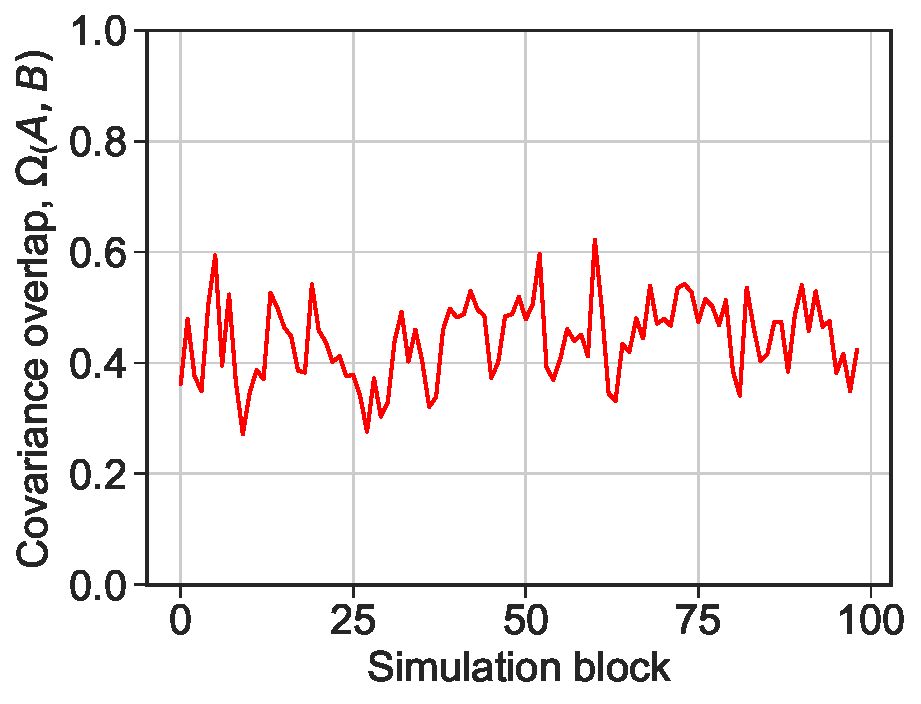
\includegraphics[width=.99\textwidth]{time_CovOver_E2.pdf}
    \caption{$E$ = 2}\label{fig:1d}
  \end{subfigure}\\%   
  \begin{subfigure}[b]{.24\linewidth}
    \centering
    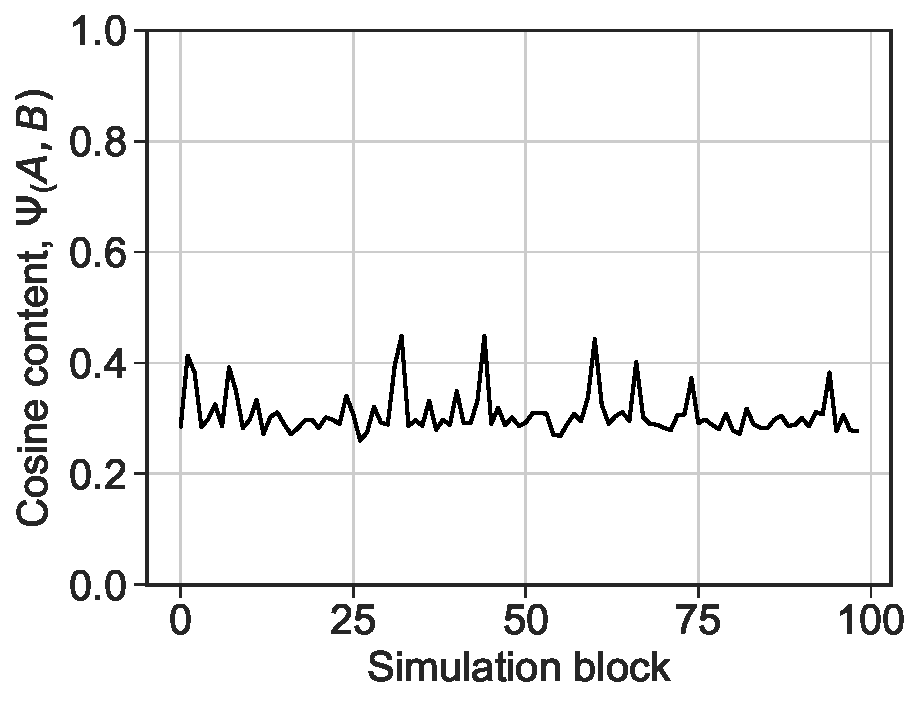
\includegraphics[width=.99\textwidth]{time_CosCont_E3.pdf}
    \caption{$E$ = 3}\label{fig:1e}
  \end{subfigure}%
  \begin{subfigure}[b]{.24\linewidth}
    \centering
    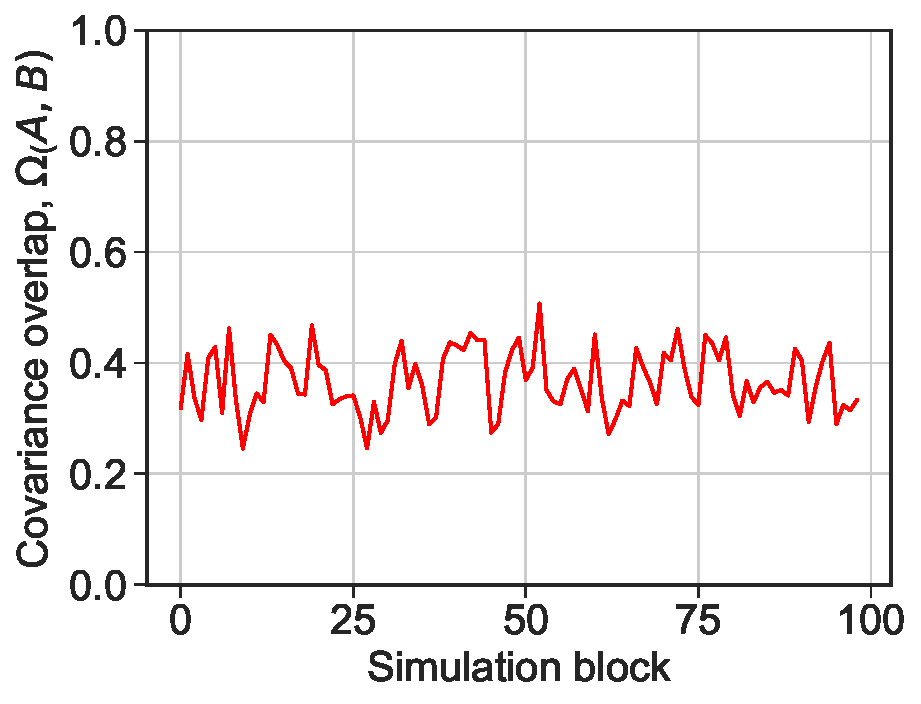
\includegraphics[width=.99\textwidth]{time_CovOver_E3.pdf}
    \caption{$E$ = 3}\label{fig:1f}
  \end{subfigure}%
  \begin{subfigure}[b]{.24\linewidth}
    \centering
    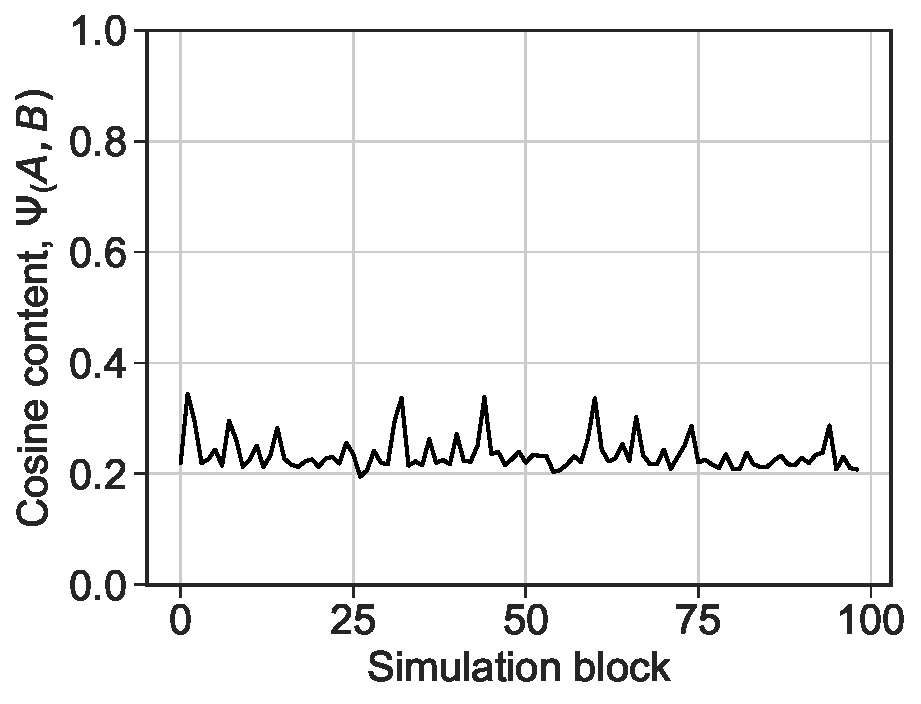
\includegraphics[width=.99\textwidth]{time_CosCont_E4.pdf}
    \caption{$E$ = 4}\label{fig:1g}
  \end{subfigure}%
  \begin{subfigure}[b]{.24\linewidth}
    \centering
    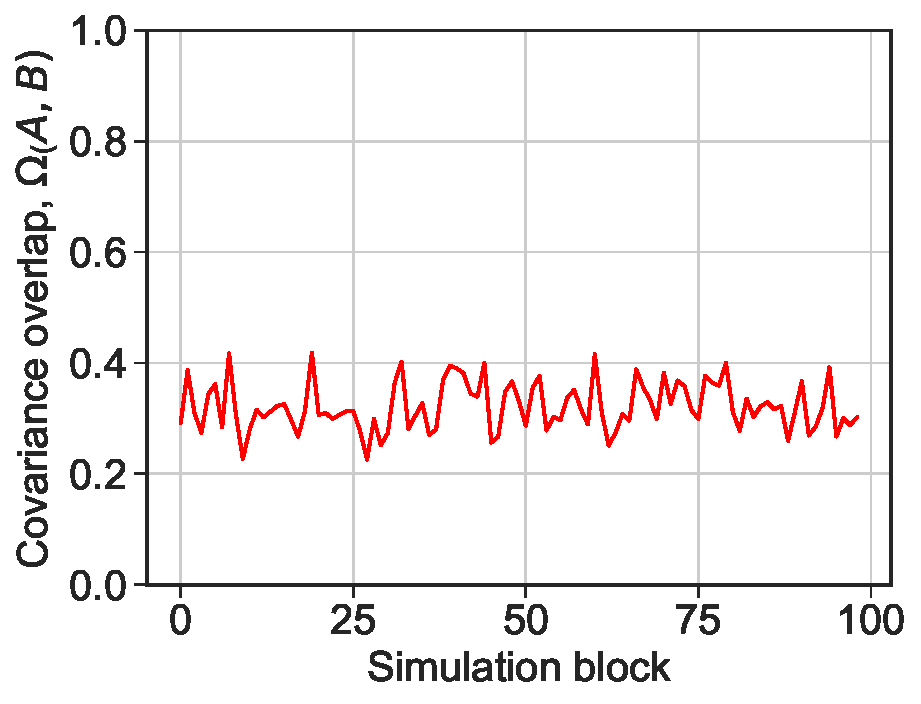
\includegraphics[width=.99\textwidth]{time_CovOver_E4.pdf}
    \caption{$E$ = 4}\label{fig:1h}
  \end{subfigure}\\%     
  \begin{subfigure}[b]{.24\linewidth}
    \centering
    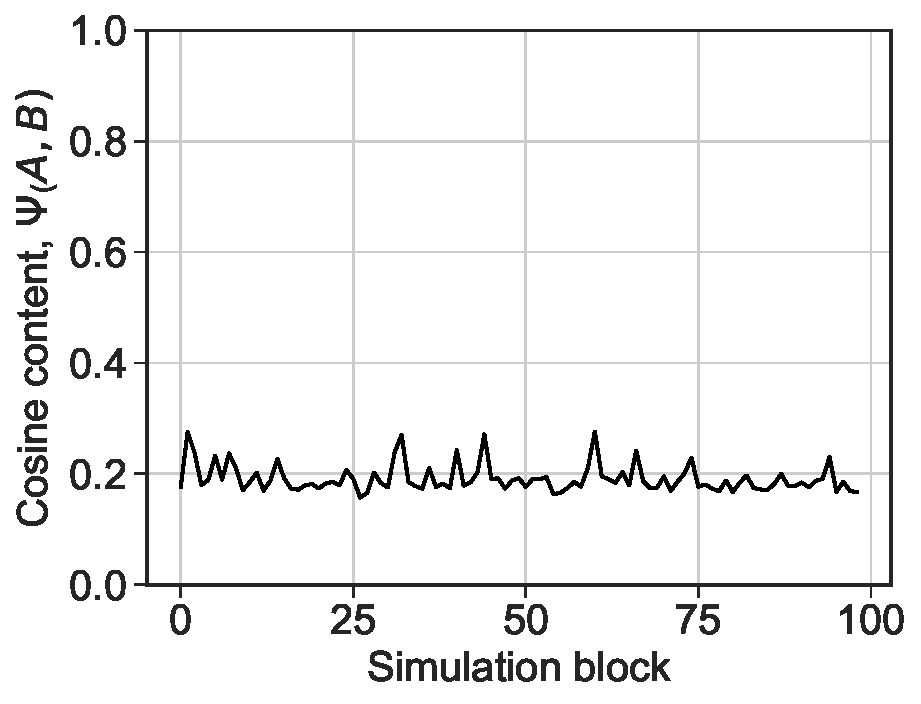
\includegraphics[width=.99\textwidth]{time_CosCont_E5.pdf}
    \caption{$E$ = 5}\label{fig:1i}
  \end{subfigure}%
  \begin{subfigure}[b]{.24\linewidth}
    \centering
    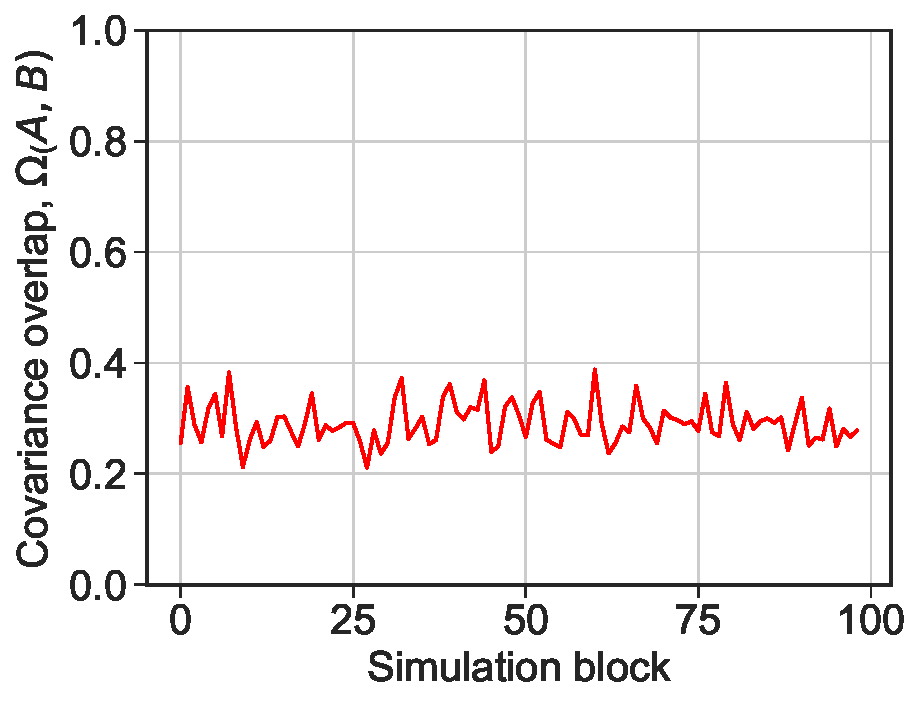
\includegraphics[width=.99\textwidth]{time_CovOver_E5.pdf}
    \caption{$E$ = 5}\label{fig:1j}
  \end{subfigure}%
  \begin{subfigure}[b]{.24\linewidth}
    \centering
    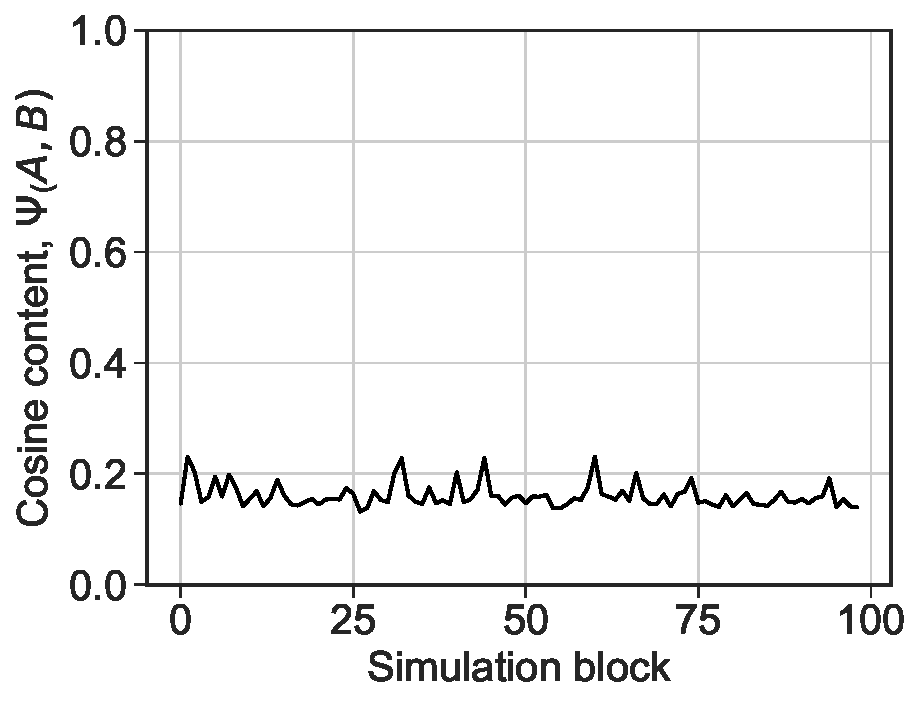
\includegraphics[width=.99\textwidth]{time_CosCont_E6.pdf}
    \caption{$E$ = 6}\label{fig:1k}
  \end{subfigure}%
  \begin{subfigure}[b]{.24\linewidth}
    \centering
    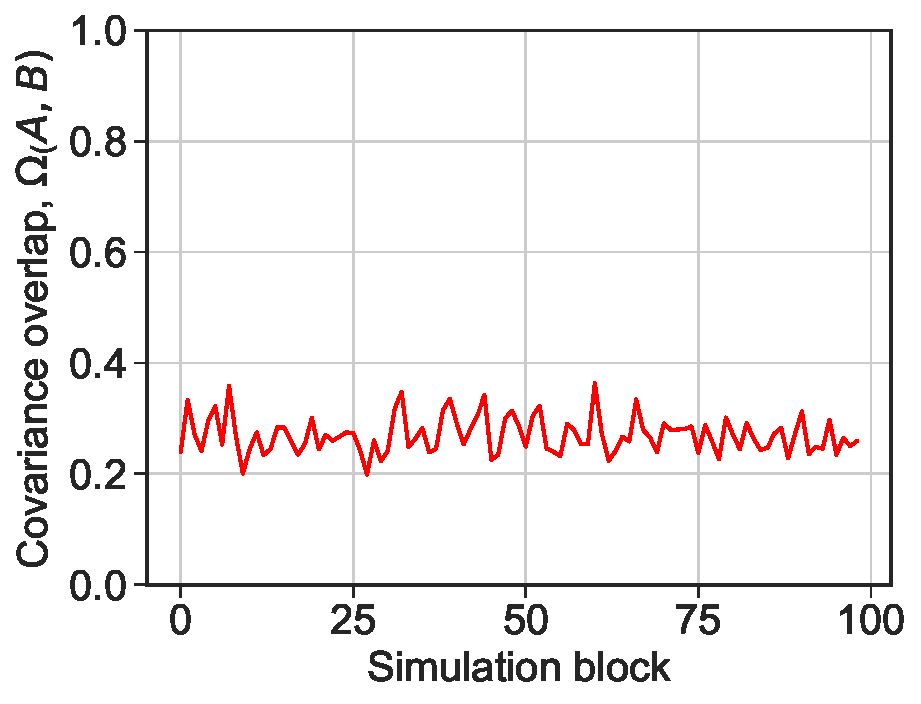
\includegraphics[width=.99\textwidth]{time_CovOver_E6.pdf}
    \caption{$E$ = 6}\label{fig:1l}
  \end{subfigure}\\%   
\caption{The numerical behaviour of spectral subspace overlap with different eigenmodes for monomeric PKM2 + Tepp-46. The MD trajectory was split into 100 blocks of 10 $ns$. The subspace overlap was calculated for each blocks $i_{n}$ and $i_{n-1}$}\label{fig:1}
\end{figure}
Similar to the deca-alanine peptide, the subspace overlap explored by the mutual information matrices of monomeric PKM2 + Tepp-46 was normally distributed about an average values of $ \Omega_{A:B} $ and $ \Psi_{A:B} $ and did not deviate as a result of the closure of the B-domain cap (shown below). Similarly, $\mu (\omega_{A:B}) $ and $\mu (\psi_{A:B}) $ decay to a convergent value, with increasing number of eigenmodes.
\begin{figure}[!ht]
\centering
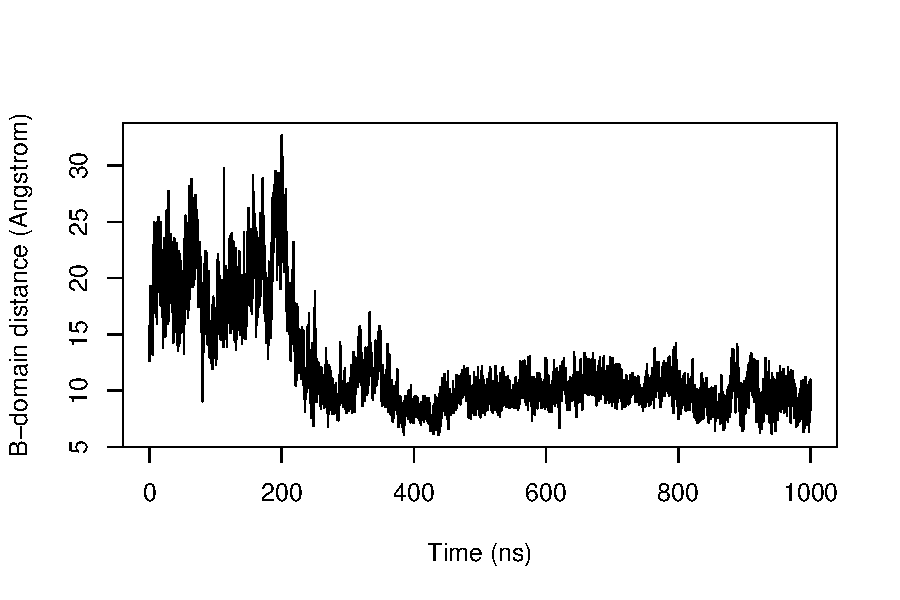
\includegraphics[scale=0.8]{distance.pdf}
\caption{The B-domain closed over the catalytic pocket of monomeric PKM2 when Tepp-46 is bound to its N-terminal allosteric pocket.}\label{fig:2} 
\end{figure}
From this, it appeared that the time evolution of backbone correlations calculated using the structural alphabet approach was not sensitive enough to pick up global structural changes. This is perhaps to be expected, because the mutual information matrices are a statistical measure of distal local correlations. Although an eigenvalue transformation of the mutual information matrices did not explicitly give information on global structural changes, we returned to the original problem of extracting meaningful correlations from the mutual information matrices. A critical question regarding the use of correlation signals is whether the signal strength observed. To filter out residual couplings from those reflecting an allosteric signal we used a random matrix theoretical framework. The fundamental aim is to detect those fragment couplings, which represents a true allosteric signal (ie. non-random). 
\end{document}
